Denne delen kan variere litt fra oppgave til oppgave. Vanligvis vil den inneholde en beskrivelse av hva som er gjort hittil pa fagfeltet man arbeider med, samt annen bakgrunnsinformasjon som er nødvendig for a forsta det arbeidet som utføres i oppgaven. En del ingeniøroppgaver vil ogsa kunne benytte matematikk (og av og til fysikk) som det ikke kan forventes at leseren skal ha intimkunnskap om pa forhand. Denne vil da beskrives her. For en studentoppgave bør det i et slikt tilfelle alltid redegjøres for all matematikk og fysikk som eventuelt benyttes.


Vi skal i denne oppgaven jobbe mye med Euler-Bernoulli modellen for materialers bøyning under påvirkning av krefter. Modellen yttrykker den vertikale forskyvningen f(x) hvor $0\leq x \leq L$. x går langs bjelken som har lengde L. Euler-Bornoulli likningen er gitt ved 
\begin{align}
    EIy''''=f(x)
\end{align}
hvor E er Youngs modulus til materialet, og I er tregheten. Begge disse er konstante langs hele bjelken. Funksjonen f(x) er er den påførte kraften, inkludert bjelkens egenvekt, per lengde-enhet. 
\\ \\
I oppgaven (Reality Check 2) har vi oppgitt formelen 2.27 og 2.28 som følger (et bevis på 2.28 kommer senere): 
\begin{align}
    EIy''''&=f(x) \nonumber \\
    y''''(x)& \approx \frac{y(x-2h)-4y(x-h)+6y(x)-4y(x+h)+y(x+2h)}{h^4}
\end{align}
Vi deler opp planken i $n$ like deler, alle med lengde $h=\frac{L}{n}$. Dette medfører at $x_0<x_1<x_2...<x_i$, hvor alle $x_i$ har lengde $h$. $x_0$ er starten på planken, $x_1$ er første steglengde ut på bjelken, $x_1=1\cdot h$. $x_2$ er på samme måte andre lengde ut på planken, $x_2=2\cdot h$. Videre blir $x_i=i\cdot h$. Hvis vi sier at $y_i=y(x_i)$ og setter dette inn i likning 2.27 får vi at 

\begin{align}
EI\cdot	\frac{y_{i-2}-4y_{i-1}+6y_i-4y_{i+1}+y_{i+2}}{h^4}=f(x)
\end{align}
Vi gjør om slik at vi får alle leddene som inneholder y på én side:
\begin{align}
    y_{i-2}-4y_{i-1}+6y_i-4y_{i+1}+y_{i+2}=\frac{h^4}{EI}f(x_i)
\end{align}
Dette er hvordan man kommer frem til likning 2.29. 
\\ \\ 
Videre skal vi bruke Euler-Bernoulli likningen på et stupebrett. Et stupebrett er en bjelke som er festet i den ene enden, og den vertikale forskyvningen på starten av brettet er naturligvis lik 0. Hvis vi bruker dette får vi følgende informasjon om starten av brettet ($y(0)$) og slutten av brettet ($y(L)$):
\begin{align}
    y(0)=y'(0)=y''(L)=y'''(L)=0
\end{align}
Men, skal vi bruke de tidligere definerte funksjonene får vi et problem. Vi ser at hvis vi har lyst til å finne den vertikale forskyvningen i det første punktet etter starten, altså $x_1$, blir dette umulig. Som sagt tidligere er $x_1=1\cdot h$, og setter vi dette inn i formelen vi tidligere har definert for den fjerdederiverte får vi: 

\begin{align}
	y''''(x_1)&\approx \frac{y((1\cdot h)-2h)-4y((1\cdot h)-h)+6y(1\cdot h)-4y((1\cdot h)+h)+y((1\cdot h)+2h)}{h^4}\nonumber \\
	y''''(x_1)&\approx \frac{y(-h)-4y(0)+6y(h)-4y(2h)+y(3h)}{h^4}
\end{align}
Bruker notasjonen $y_i=y(x_i)$, hvor $x_i$ er som før, får vi at: 

\begin{align}
    y_{-1}-4y_0+6y_1-4y_2+y_3&=\frac{h^4}{EI}f(x_1)
\end{align}
Det er her vi har et problem. $y_{-1}$ er ikke definert grunnet at vi har ingen punkter som kommer før stupebrettets begynnelse. Derfor trenger vi et nytt uttrykk for $y''''(x)$ som gjelder bare for $x_1=1 \cdot h$. Dette uttrykket er som følger (bevis kommer senere) : 

\begin{align}
    y''''(x_1) &\approx \frac{16y(x_1)-9y(x_1+h)+\frac{8}{3}y(x_1+2h)-\frac{1}{4}y(x_1+3h)}{h^4}
\end{align}

Vi har altså et generelt uttrykk for $y''''(x)$, med et unntak for $y(x_1)$. Dette er, som sagt før: 
\begin{align}
     y''''(x)& \approx \frac{y(x-2h)-4y(x-h)+6y(x)-4y(x+h)+y(x+2h)}{h^4}
 \end{align} 
 Som vi ser av dette uttrykket bruker det punktene $x+h$ og $x+2h$. Vi har altså litt av det samme problemet som vi hadde for $x_1$: På slutten av planken, ved $x=L$, vil uttrykket inneholde punktene $L+h$ og $L+2h$. Vi har altså 2 punkter som er lengre enn brettets lengde, og derfor trenger vi nye uttrykk for $y''''(x_{n-1})$ og $y''''(x_n)$. Disse er som følger (skal ikke bevises, antas som gyldige): 
\begin{align}
    y''''(x_{n-1})&\approx \frac{-28y_n+72y_{n-1}-60y_{n-2}+16y_{n-3}}{17h^4} \\
    y''''(x_n)&\approx \frac{72y_n-156y_{n-1}+96y_{n-2}-12y_{n-3}}{17h^4}
\end{align}

Vi har nå gyldige uttrykk for hele plankens lengde. I bokas likning/figur 2.34 er matrisen som avbildet i figur \ref{fig:EBMatrix}. 
\begin{figure}[h]
    \centering
    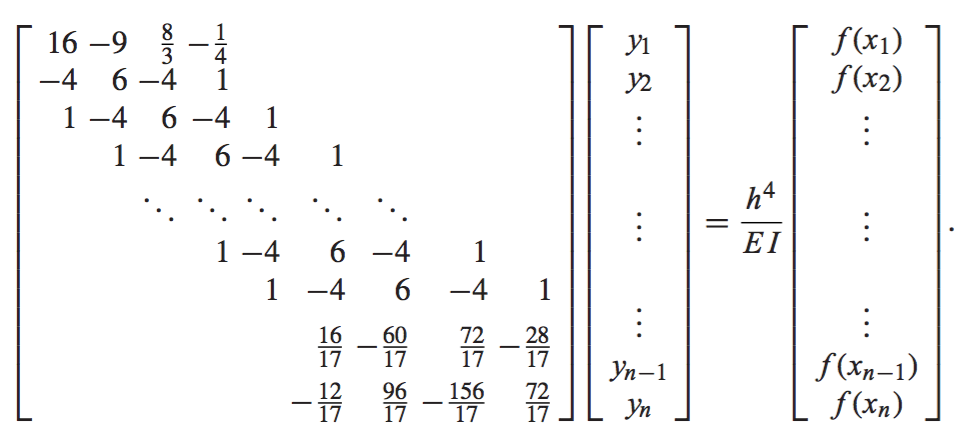
\includegraphics[width=0.8\textwidth]{sections/Theory/EBMatrix}
    % 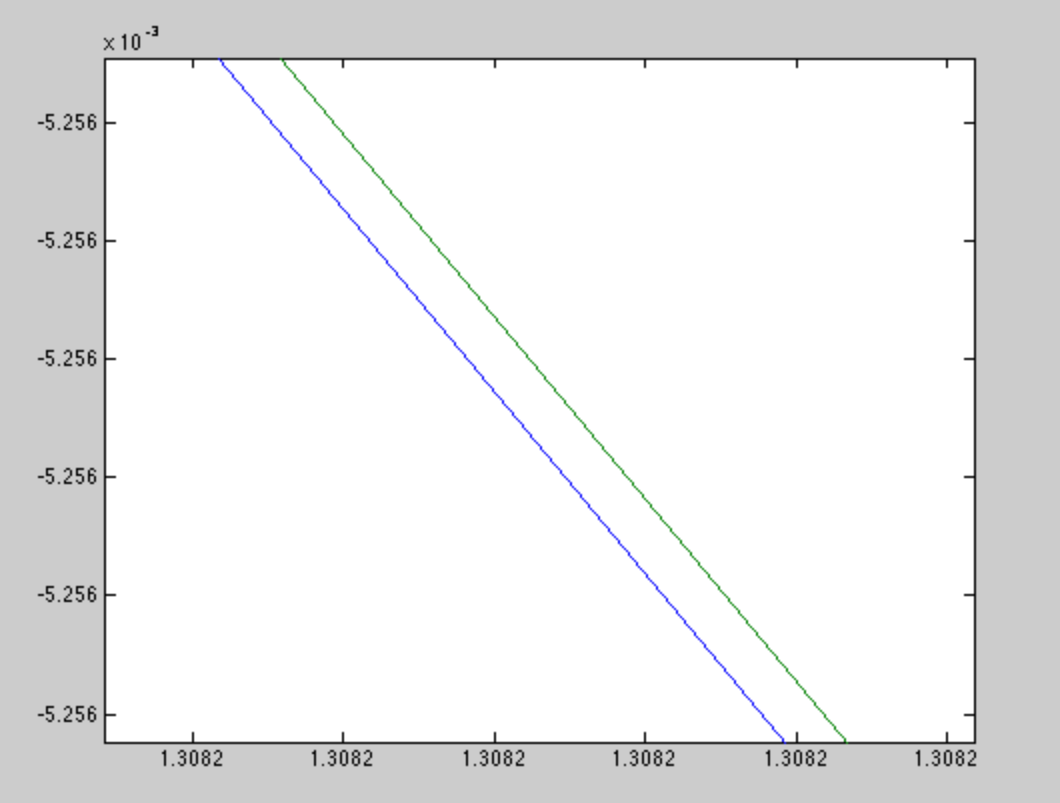
\includegraphics[width=0.8\textwidth]{errorplot2}
    \caption{Matrisen 2.34 fra boken}
    \label{fig:EBMatrix}
\end{figure}
Tallene i denne matrisen stemmer godt med likningene vi har funnet. Likningen for $x_1$ hadde koeffisientene 16, -9, $\frac{8}{3}$ og $-\frac{1}{4}$, og dette stemmer overens med første linje i matrisen. Resten av matrisen, frem til de 2 siste leddene, skulle ha koeffisientene 1, -4, 6, -4 og 1. Linje 2, altså $x_2$, har koeffisientene -4, 6, -4 og 1. Dette er fordi det generelle uttrykket er 

\begin{align}
    y''''(x)& \approx \frac{y(x-2h)-4y(x-h)+6y(x)-4y(x+h)+y(x+2h)}{h^4} \nonumber
\end{align}
og i $x=2h$ er $y((2\cdot h)-2h)=y(0)=0$. De 2 siste linjene i matrisen stemmer overens med uttrykkene vi fant for $y''''(x_{n-1})$ og $y''''(x_n)$. 
\\ \\
Følgende kommer et bevis på at den fjerdederiverte (likning 2.28) kan approksimeres ved: 

\begin{align}
    f^{iv}(x)=\frac{f(x-2h)-4f(x-h)+6f(x)-4f(x+h)+f(x+2h)}{h^4}\nonumber
\end{align}

Først setter vi opp taylor-rekker for punktene $x+2h$, $x-2h$, $x+h$, $x-h$: 
\begin{align}
    f(x+2h)&=f(x)+2hf'(x)+2h^2f''(x)+\frac{(4h)^3}{3!}f'''(x)+\frac{(2h)^4}{4!}f^{(4)}(x)+\frac{(2h)^5}{5!}f^{(5)}(x)+h^6\nonumber\\ 
    f(x-2h)&=f(x)-2hf'(x)+2h^2f''(x)-\frac{(4h)^3}{3!}f'''(x)+\frac{(2h)^4}{4!}f^{(4)}(x)-\frac{(2h)^5}{5!}f^{(5)}(x)+h^6\nonumber\\
    f(x+h)&=f(x)+hf'(x)+\frac{h^2f''(x)}{2}+\frac{h^3}{3!}f'''(x)+\frac{h^4}{4!}f^{(4)}(x)+\frac{h^5}{5!}f^{(5)}(x)+h^6\nonumber\\
    f(x-h)&=f(x)-hf'(x)+\frac{h^2f''(x)}{2}-\frac{h^3}{3!}f'''(x)+\frac{h^4}{4!}f^{(4)}(x)-\frac{h^5}{5!}f^{(5)}(x)+h^6\nonumber
\end{align}

Deretter legger vi først sammen $f(x+2h)$ og $f(x-2h)$: 

\begin{multline}
    \\
    f(x+2h)+f(x-2h)= \\
    f(x)+2hf'(x)+2h^2f''(x)+\frac{(4h)^3}{3!}f^3(x)+\frac{(2h)^4}{4!}f^{4}(x)+\frac{(2h)^5}{5!}f^{(5)}(x)+h^6 \\
    + \\
  	f(x)-2hf'(x)+2h^2f''(x)-\frac{(4h)^3}{3!}f^3(x)+\frac{(2h)^4}{4!}f^{4}(x)-\frac{(2h)^5}{5!}f^{(5)}(x)+h^6\nonumber \\
  	=\\
  	2f(x)+4h^2f''(x)+\frac{4}{3}h^4f^{(4)}(x)+h^6 \nonumber\\
\end{multline}

Deretter legger vi sammen $f(x+h)$ og $f(x-h)$: 
\begin{multline}
	f(x)+hf'(x)+\frac{h^2f''(x)}{2}+\frac{h^3}{3!}f'''(x)+\frac{h^4}{4!}f^{(4)}(x)+\frac{h^5}{5!}f^{(5)}(x)+h^6\\
	+\\
	f(x)-hf'(x)+\frac{h^2f''(x)}{2}-\frac{h^3}{3!}f'''(x)+\frac{h^4}{4!}f^{(4)}(x)-\frac{h^5}{5!}f^{(5)}(x)+h^6\\
	=\\
	2f(x)+h^2f''(x)+\frac{h^4f^{(4)}(x)}{12} + h^6 \nonumber \\
\end{multline}

Til slutt legger vi sammen $f(x+h)+f(x-h)$ og $\frac{f(x+2h)+f(x-2h)}{-4}$: 
\begin{multline}
	\\
	2f(x)+h^2f''(x)+\frac{h^4f^{(4)}(x)}{12} + h^6 \\
	+\\
	\frac{2f(x)+4h^2f''(x)+\frac{4}{3}h^4f^{(4)}(x)+h^6 }{-4}\\
	=\\
	\frac{3}{2}f(x)-\frac{3}{12}h^4f^{(4)}(x)+h^6\\
\end{multline}

Deretter løser vi likningen med hensyn på $f^{(4)}(x)$: 
\begin{align}
    f(x+h)+f(x-h)-\frac{f(x+2h)}{4}-\frac{f(x-2h)}{4}=\frac{3}{2}f(x)-\frac{3}{12}h^4f^{(4)}(x)+h^6\nonumber
\end{align}
\begin{align}
     -3h^4f^{(4)}(x)&=12f(x+h)+12f(x-h)-3f(x+2h)-3f(x-2h)-18f(x) +h^6 \nonumber \\
     \nonumber \\
	f^{(4)}(x)&=\frac{-4f(x-h)+f(x-2h)+6f(x)+f(x+2h)-4f(x+h)}{h^4}
\end{align}
 

Her kommer det andre beviset: 
\begin{align}
f(x+2h)+f(x-2h)+f(x+h)+f(x-h)=f4(x)+5h^2f''(x)+\frac{17}{12}h^{(4)}(x)+h^6 \nonumber
\end{align}

Vi setter $f^{(4)}$ alene, og får: 

\begin{align}
	f^{(4)}=\frac{12f(x+2h)}{17h^4}+\frac{12f(x-2h)}{17h^4}+\frac{12f(x+h)}{17h^4}+\frac{12f(x-h)}{17h^4}-\frac{48f(x)}{17h^4}-\frac{60f''(x)}{17h^2}+\frac{h^6}{h^4}
\end{align}

Vi ser at vi trenger $f''(x)$. HER SKAL VI FINNE DEN; HVORDAN GJØR VI DET?!??!?!?! 
Setter vi dette inn i uttrykket vi har for $f^{(4)}(x)$ får vi: 

\begin{multline}
    f^{(4)}(x)=\frac{12f(x+2h)}{17h^4}+\frac{12f(x-2h)}{17h^4}+\frac{12f(x+h)}{17h^4}+\frac{12f(x-h)}{17h^4}-\frac{48f(x)}{17h^4}-\\ \frac{60f}{17h^2}\cdot (\frac{-f(x+2h)+16f(x+h)-30f(x)+16f(x-h)-f(x-h)}{12h^2})+\frac{h^6}{h^4} \nonumber
\end{multline}

\begin{multline}
    f^{(4)}(x)=\frac{12f(x+2h)}{h^4}+\frac{12f(x-2h)}{h^4}+\frac{12f(x+h)}{h^4}+\frac{12f(x-h)}{h^4}-\frac{48f(x)}{h^4} \\
    +\frac{5f(x+2h)}{17h^4}-\frac{80f(x+h)}{17h^4}+\frac{150f(x)}{17h^4}-\frac{80f(x-h)}{17h^4}+\frac{5f(x-2)}{17h^4} + \frac{h^6}{h^4} \nonumber
\end{multline}

\begin{align}
    f^{(4)}(x)&=\frac{f(x+2h-4f(x+h)+6f(x)-4f(x-h)+f(x-2h)}{h^4} + h^2
\end{align}